\chapter{Enhanced Rotation-Equivariant U-Net for Nuclear Segmentation}
\label{chap-method}
\begin{ChapAbstract}
In this chapter, we present our proposed method for nuclear segmentation in H\&E stained histopathology images. Specifically, we consider enforcing rotation equivariance in the network, the placement of residual blocks, and applying novel data augmentation designed specifically for histopathology images, and show the relative improvement and merit of each. Incorporating all of these enhancements in the design and training of a U-Net yields significantly improved segmentation results while still maintaining a speed of inference that is sufficient for realworld applications, in particular, analyzing whole-slide images (WSIs).  
\end{ChapAbstract}

\section{Overview of proposed methods}
The recent surge in interest in deep learning coupled with increasing availability of large-scale histopatholical image data sets, such as The Cancer Genome Atlas \cite{tcga}, has resulted in significant advances in computational histological analysis \cite{he_dataset_kumar, unet}. A crucial step in such analysis pipelines is accurate and efficient segmentation of cell nuclei \cite{review_seg_overall}. With the aid of large-scale training data, deep-learningbased methods for automatically segmenting nuclei have surpassed traditional approaches, such as watershed \cite{watershed}
and thresholding \cite{Otsu} algorithms, though, despite these improvements, this step remains challenging and continues to be an active area of research \cite{review_seg_overall}. Changes in nuclear morphology are well-studied indicators of diseases, such as cancer, which motivates the continued development of effective methods of automated segmentation.

Initial approaches using deep learning operated by scanning the image patch-by-patch and generating a label (e.g., nucleus or non-nucleus) for each pixel centered in each patch \cite{he_dataset_kumar}. Subsequent morphological processing could be applied to help smooth and refine the generated label masks and ensure that the segmented regions are contiguous. More recently, the U-Net architecture was proposed \cite{unet}, which operates on the entire image and jointly infers the label at each pixel simultaneously, leading to more spatially coherent segmentation. U-Nets have been shown to achieve improved accuracy on several bioimage segmentation tasks, even when the data set is relatively small \cite{unet}.

In this work, we bring together several recent developments in bioimage analysis to enhance the current methodology for deep-learning-based nuclear segmentation and, through a thorough ablation study, show the relative improvement and merit of each. We show that combining these enhancements together can achieve significantly improved scores for several important metrics at a speed that
is sufficient for real-world applications, such as analyzing
whole-slide images (WSIs). In more detail, enforcing rotation equivariance in the network, the placement of residual blocks, and applying novel data augmentation designed
specifically for histopathology images are proven to overcome challenges not only in nuclear segmentation but also other related domains such as astronomy data through the relative improvements. Section \ref{sec:main_challenges} discusses the main challenges not only in the nuclear segmentation field but also other related domains as well as overview of our enhancements to overcome these problems. The merit of each enhancement will be described in more detail in section \ref{sec:proposed_method}. 

\section{Main indicated challenges}
\label{sec:main_challenges}
\subsection{Equivariance to rotation \& translation group}

As proven in \cite{gcnn}, the convolutional neural networks are effective because of weight sharing mechanism, which activates the translation symmetry in most perception task. It means that the feature of shifted version of image feeded to the network is same as the shifted feature of the original images plugged to the same network. However, when it comes to other transformation such as rotation, reflection, etc. the designed architecture fail to maintain such equivariance properties. This limits the generalization of the results produced from these kind of architectures, especially in many filed such as microscopy image segmentation, astronomy analysis, ... To overcome this challenge, especially in nuclear segmentation problem, the first enhancement to the U-Net we consider is to encode equivariance to groups, specifically rotation and translation, following the work of group-equivariant CNNs (GCNNs) \cite{gcnn}, thereby obviating the need to learn such equivariance through extensive and time-consuming data augmentation. This enhancement helps the learned network to better generalize to such variation in unseen data. G-CNNs have recently been shown to demonstrate top performance on segmenting regions of interest in histology images \cite{DBLP:journals/corr/abs-1806-03962} and biological structures in other types of bioimages \cite{DBLP:journals/corr/abs-1804-03393}, but have not yet been applied to the task of nuclear segmentation.

\subsection{Limited receptive field for boundary classification}

\begin{figure}[thb]
    \centering
    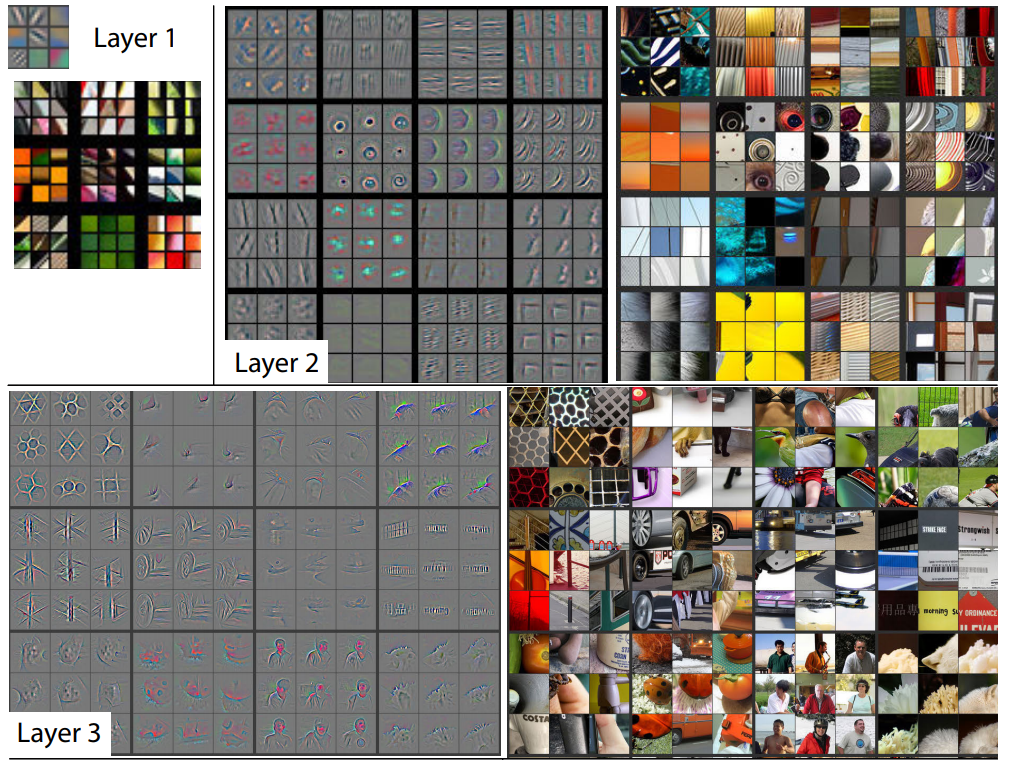
\includegraphics[width=\textwidth]{resources/5_feautures.png}
    \caption{Each layers of networks \cite{ZFNet} are responsible for detecting a type of features (including low-level and high-level one).}
    \label{fig:low_high_features}
\end{figure}

As visualized in figure \ref{fig:low_high_features} from \cite{ZFNet}, the earlier layers of convolutional neural networks are responsible for detecting low-level features such as contour, edge, while the deeper layers detect high-level features like eyes, noses, etc. As this results, the low-level branches of U-Net, which have limited receptive field, focus on analyzing the contours or edges existing in the data. This phenomenon affects a lot on problems require segmenting accurately on the boundary, for example in nuclear segmentation. In this type of problem, to segment correctly the boundary, the network needs to expand its receptive field of these low-level layers to have more information to decide whether the current pixel belongs to boundary class. Therefore, we decide to enhance the long-skip connections in the U-Net from the downsampling to upsamling arms of the “U” with residual blocks, an insight that has shown improved performance for other applications \cite{DeepLabv1}. The motivating hypothesis of this modification is that providing richer low-level features from the downsampling arm, learned through the residual blocks, to the upsampling arm will aid in producing detailed boundaries, especially between touching nuclei. This enhancement is not limited to nuclear segmentation problems but all tasks requiring the accurate boundary segmentation. 

\subsection{Data shortage}

Lastly, we propose a novel means of data augmentation specifically designed for histological images to aid in training. Although the rate of generation of H\&E image data is increasing, fully-labeled training data is still scarce. Therefore, augmentation of training data is still crucial for learning robust models. In addition to standard augmentation techniques of elastic deformations, blurring, and additive noise, we generate synthetic images by slightly translating and deforming the nuclei and filling any empty pixels by inpainting \cite{DBLP:journals/corr/abs-1801-07892}. This method was inspired by recent work in video object segmentation \cite{DBLP:journals/corr/KhorevaBIBS17}, which demonstrated significant improvements in performance. Others works have also proposed means of generating synthetic, realistic histological images \cite{DBLP:journals/corr/abs-1810-00236}, though ours is much simpler to implement. Although this scheme is specialized for nuclear segmentation in H\&E stained histopathology images, it could be applied for other domains such as other microscopy data, video data, etc.

\section{Methods}
\label{sec:proposed_method}
The standard U-Net architecture consists of two arms, one for downsampling the feature maps to a lower-dimensional space and one for upsampling the feature maps back to full resolution.
Each downsampling layer consists of convolution, non-linear activation, pooling, and batch normalization.
Each upsampling layer consists of similar operations except that pooling is replaced by upsampling.
Additionally, residual blocks~\cite{Resnet}, which are used to increase the depth of the network, can be added.
In~\cite{DBLP:journals/corr/HanKK16}, some experiments evaluated the performance of different types of residual blocks.
We inherit from their work the architecture producing the best reported performance. 
Lastly, to help with interpolating the higher-resolution feature maps, features from the downsampling arm are conveyed to the upsampling layers by long-skip connections.
From this baseline architecture, we incorporate two enhancements, namely group-equivariant operations to encode equivariance to rotation and translation, and residual blocks along the long-skip connections.
We describe these enhancements below.

As in other deep-learning-based approaches~\cite{he_dataset_kumar}, we formulate nuclear segmentation as a pixel labeling problem with three potential labels, namely, nuclear interior, nuclear boundary, and background.
The network is designed and trained to produce a probability map for each label.
Creating a label especially for the boundary results in a larger contribution to the objective for boundary pixels and thereby encourages the network to produce a more accurate boundary, which is generally harder to infer by post-processing than pixels away from nuclear boundaries.
Our post-processing method of morphological operations, described below, helps to refine the output of the U-Net by smoothing edges and ensuring contiguous segmentation boundaries.

Input data is first stain-normalized before being fed to the U-Net.
To help train the model, we employ several means of data augmentation, including our proposed histology-specific method, which we describe below. 

\subsection{Encoding group-equivariance}

As noted in~\cite{gcnn}, it is helpful to think of the input image to a neural network as a function $f\colon\mathbb{Z}^{2}\rightarrow \mathbb{R}^{K}$ that maps 2D space to pixel intensities.
The insight of~\cite{gcnn} for CNNs was to generalize equivariance to translation, which is inherent to standard convolution, to other transformations by defining convolution for \emph{groups} in general, of which $\mathbb{Z}^{2}$ with translations is a specific example.
An important group for histology images is the $p4$ group, which consists of translations and rotations about the origin by 90 degrees of elements in $\mathbb{Z}^{2}$.
%and a filter $\psi^{i}\colon\mathbb{Z}^{2}\rightarrow \mathbb{R}^{K}$, both of which operate on the 2D space of integers
A group-equivariant neural network can be created by the composition of group-equivariant convolution with several other group operations, given below, which preserve equivariance to such transformations throughout the network.
The placement of these operations in the network can be seen in Figure~\ref{fig:g_u_net}. 

\begin{figure}[thb]
    \centering
    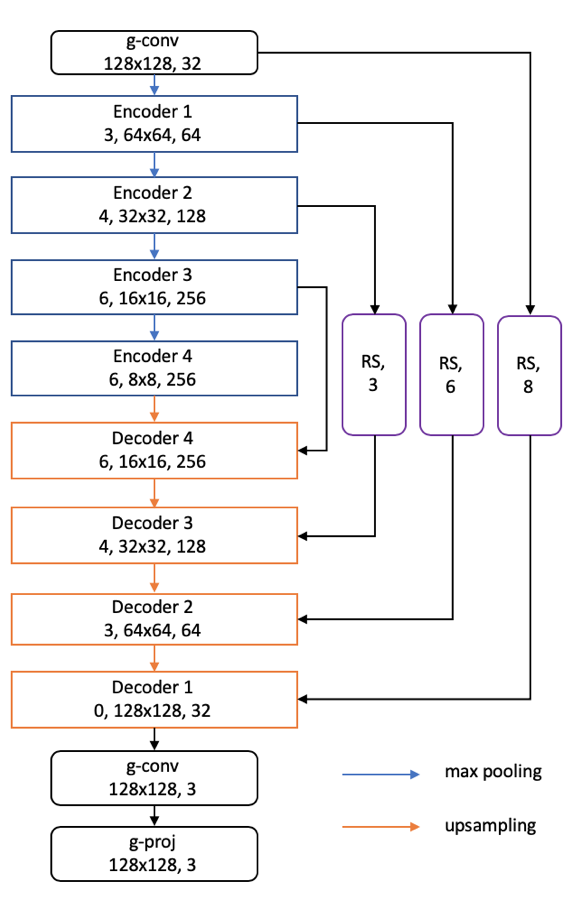
\includegraphics[scale=0.95]{resources/4_UNet_Architecture-part1.png}
    \caption{Our proposed rotation and translation-equivariant U-Net architecture at the 
    highest-level view, showing sequential encoder and decoder blocks.}
    \label{fig:g_u_net}
\end{figure}

Our residual blocks along the long-skip connections of low-level layers are also shown in Figure~\ref{fig:g_u_net_details}: (a) details of encoder blocks; (b) details of decoder blocks;     (c) details of RS blocks, with several residual blocks in series, which are found on long-skip connections and within decoder and encoder blocks; and (d) details of residual blocks. Because of limited space, we omit the visualization of batch normalization layers and ReLu activation layers after g-conv blocks. 

\begin{figure}[thb]
    \centering
    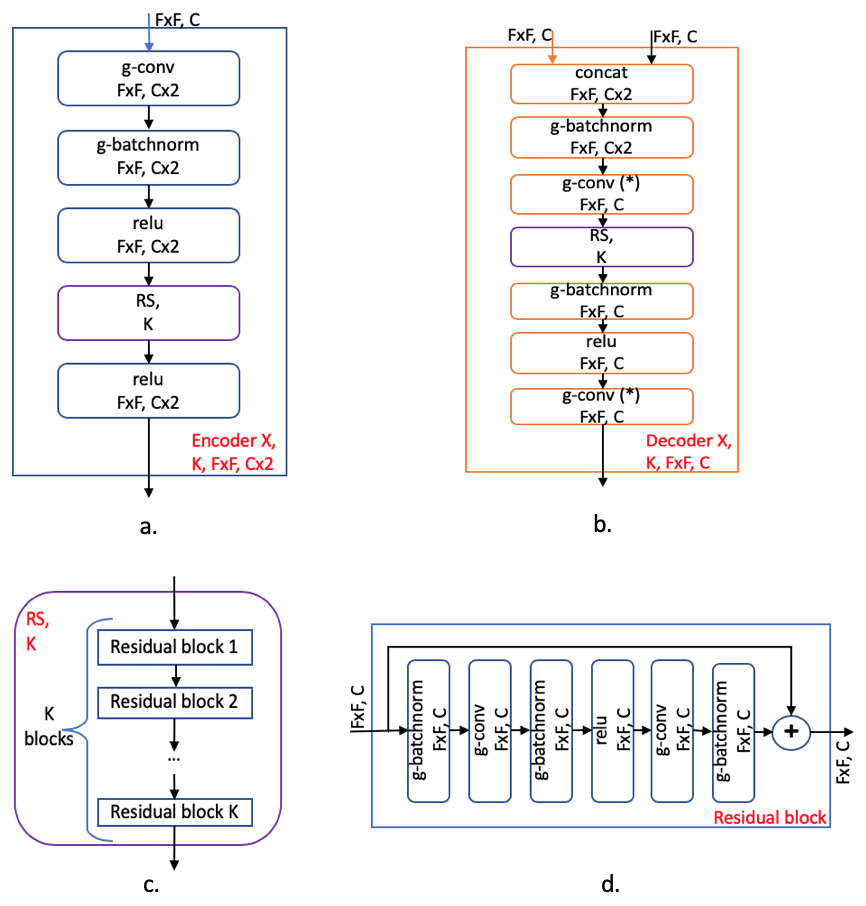
\includegraphics[scale=0.95]{resources/4_UNet_Architecture-part2.png}
    \caption{Residual blocks along the long-skip connections of low-level layers.}
    \label{fig:g_u_net_details}
\end{figure}

\subsubsection*{Group-equivariant convolution}
Group-equivariant convolution is the generalization of convolution to functions on groups, the set $\mathbb{Z}^{2}$ with translation, on which convolution is normally defined, being a specific type of group.
For a group $G$, the convolution of a filter $\psi\colon G\rightarrow \mathbb{R}^{K}$ with a feature map $f\colon G\rightarrow \mathbb{R}^{K}$  is defined to be the sum, over all elements in $G$, of their inner product:
\begin{equation}
    (f\ast \psi)(g) = \sum_{k}\sum_{h\in G} f_{k}(h)\psi_{k}(g^{-1}h).
\end{equation}
Here, the action of element $g$ on $h\in G$ is expressed by $gh$, and $g^{-1}h$ is the action of the inverse of $g$.
For example, if the group is the translation of elements $x\in\mathbb{Z}^{2}$, then $gx = x + g$ and $g^{-1}x = x - g$ and we would have standard convolution.
Since the output function is a function of $G$, which indexes not only pixel locations, but also rotations, this information can be preserved throughout the network thereby preserving equivariance to such transformations.

Since the input images to the network are functions on $\mathbb{Z}^{2}$, the output of the first group-equivariant convolutional layer is a special case, given by
\begin{equation}
    (f\ast \psi)(g) = \sum_{k}\sum_{z\in \mathbb{Z}^{2}} f_{k}(z)\psi_{k}(g^{-1}z).
\end{equation}

\subsubsection*{Group-equivariant upsampling}

For the upsampling arm of the U-Net, before each layer, we first upsample the feature map from the layer below by 2 using nearest-neighbor interpolation, which preserves equivariance to translations and rotations of 90 degress.
This method of upsampling is the same as \emph{deconvolution} or \emph{transpose} convolution with a $2 \times 2$ filter of all ones~\cite{FCNs} and helps to keep the number of trainable filters in the network manageable.
%For the upsampling arm of the U-Net, convolution is replaced with \emph{deconvolution}, or \emph{transpose} convolution.
%Deconvolution in the context of a U-Net is accomplished by first interpolating the feature map uniformly with zeros so that it is the desired dimension, and then convolving~\cite{long2015fully}.
%As noted in~\cite{linmans2018sample}, this operation maintains group equivariance for $p4m$, regardless of the stride.

\begin{figure}[thb]
\begin{center}
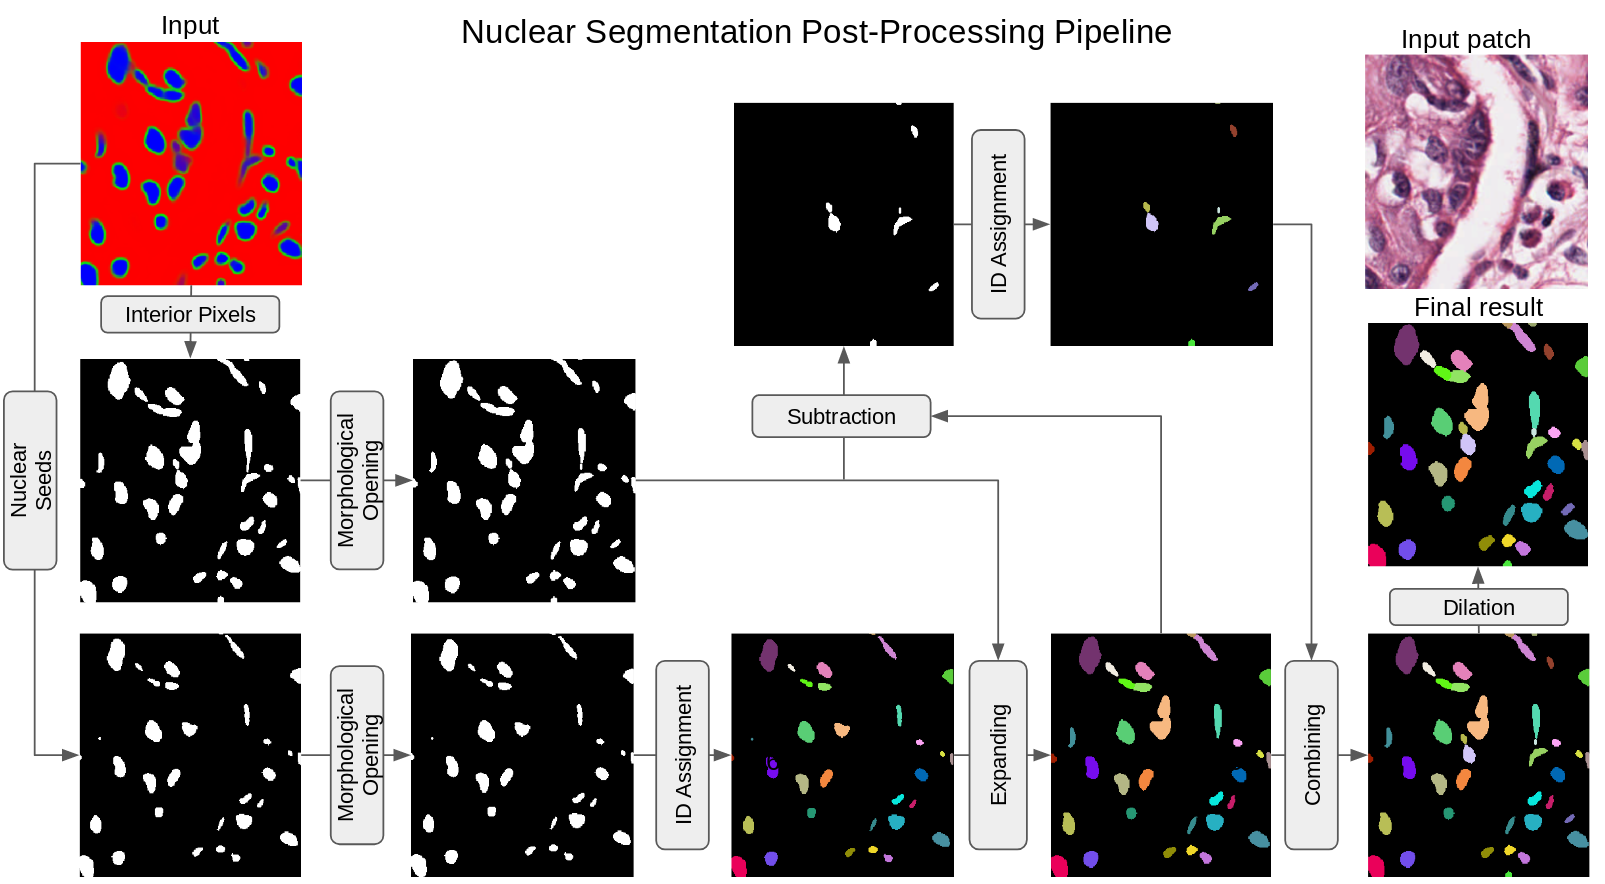
\includegraphics[width=\textwidth]{resources/4_post_processing.png}
\end{center}
   \caption{Our proposed post-processing method, consisting of a series of several morphological operations.
   Each step is visualized by its result.}
\label{fig:post_processing}
\end{figure}

\subsubsection*{Group-equivariant pooling and residual blocks}

As noted in~\cite{gcnn}, for the $p4$ group, max-pooling with a stride of 2 preserves the equivariance properties of the network, and this is the pooling operation we use in the downsampling arm of the U-Net.
Also noted in~\cite{gcnn}, since residual blocks are simply the addition of two group-equivariant feature maps, the output will also be group-equivariant.

\subsubsection*{Group projection}
To create the final segmentation image, we must transform the domain of the feature maps in the U-Net from $G$ back to $\mathbb{Z}^{2}$.
To do so, we average the feature map for each filter over rotations.
This is called the group \emph{projection} layer, as in other works~\cite{DBLP:journals/corr/abs-1807-00583}.

\subsection{Long-skip connections with residual blocks}
In the typical U-Net~\cite{unet} architecture, the number of convolution blocks at low-level layers is small, which limits the effective local field-of-view and thereby decreases the quality of features which the network can use to delineate the output boundary.
To provide richer low-level features to the final layers of the upsampling arm of the U-Net, we enhanced the baseline U-Net by adding residual blocks on long-skip connections.
Our long-skip connections enhanced with residual blocks are visualized in Figure~\ref{fig:g_u_net}a, and a detailed view of the long-skip connections and residual blocks are shown in Figure~\ref{fig:g_u_net}d and Figure~\ref{fig:g_u_net}e, respectively.

\subsection{Morphological post-processing}

Even though the U-Net deep learning architecture produces a full segmentation mask, unlike patch-based deep learning methods, post-processing, specifically morphological operations, are still essential to yielding contiguous regions and accurate nuclear boundaries.
%To aid the network in learning invariance to rotations and flips, each image is manipulated by rotations of 90 degrees and vertical flipping and the result of the network for all eight orientations is averaged to yield a single map indicating the probability of each pixel belonging to each label.
We designed a post-processing pipeline, shown in Figure~\ref{fig:post_processing}, to accomplish this.
It consists of the following steps.
A mask of confident interior pixels is created by identifying pixels for which the inside probability is greater than other labels, followed by morphological opening.
A map of nuclear seeds is created by thresholding ($thres = 0.85$) the probability of the interior class of these pixels, followed by opening.
Each seed is assigned a unique index, which is propagated to all connected interior pixels.
Regions not covered will be assigned new index and combined with the previous result.
Then, we apply binary dilation to create the final result.
The parameters, such as window size, for these various morphological operations were optimized on the validation set in our experiments.

%\begin{figure}[t]
%\begin{center}
%\includegraphics[width=0.42\textwidth]{image/img_new_synthetic_normalized_edit.png}
%\end{center}
%   \caption{Data augmentation and color normalization. The first row shows example training images from~\cite{kumar2017dataset}.
%   The second row shows synthetic images generated by our proposed data-augmentation method.
%   %New shape and orientation of nuclei eyes generated along with translation, which increases the overlapping rate, make the training set more diverse. These new synthetic images have a significant contribution to the performance. 
%   The last row shows the original training images normalized by method proposed in~\cite{7164042}. \CC{[TODO: merge with Figure 4]}} 
%   %By converting all images to one color space, we can reduce the color variance problem, which alleviates the challenge when the model is trained.}
%\label{fig:data_visualize}
%\end{figure}
%

\begin{figure}[thb]
    \centering
    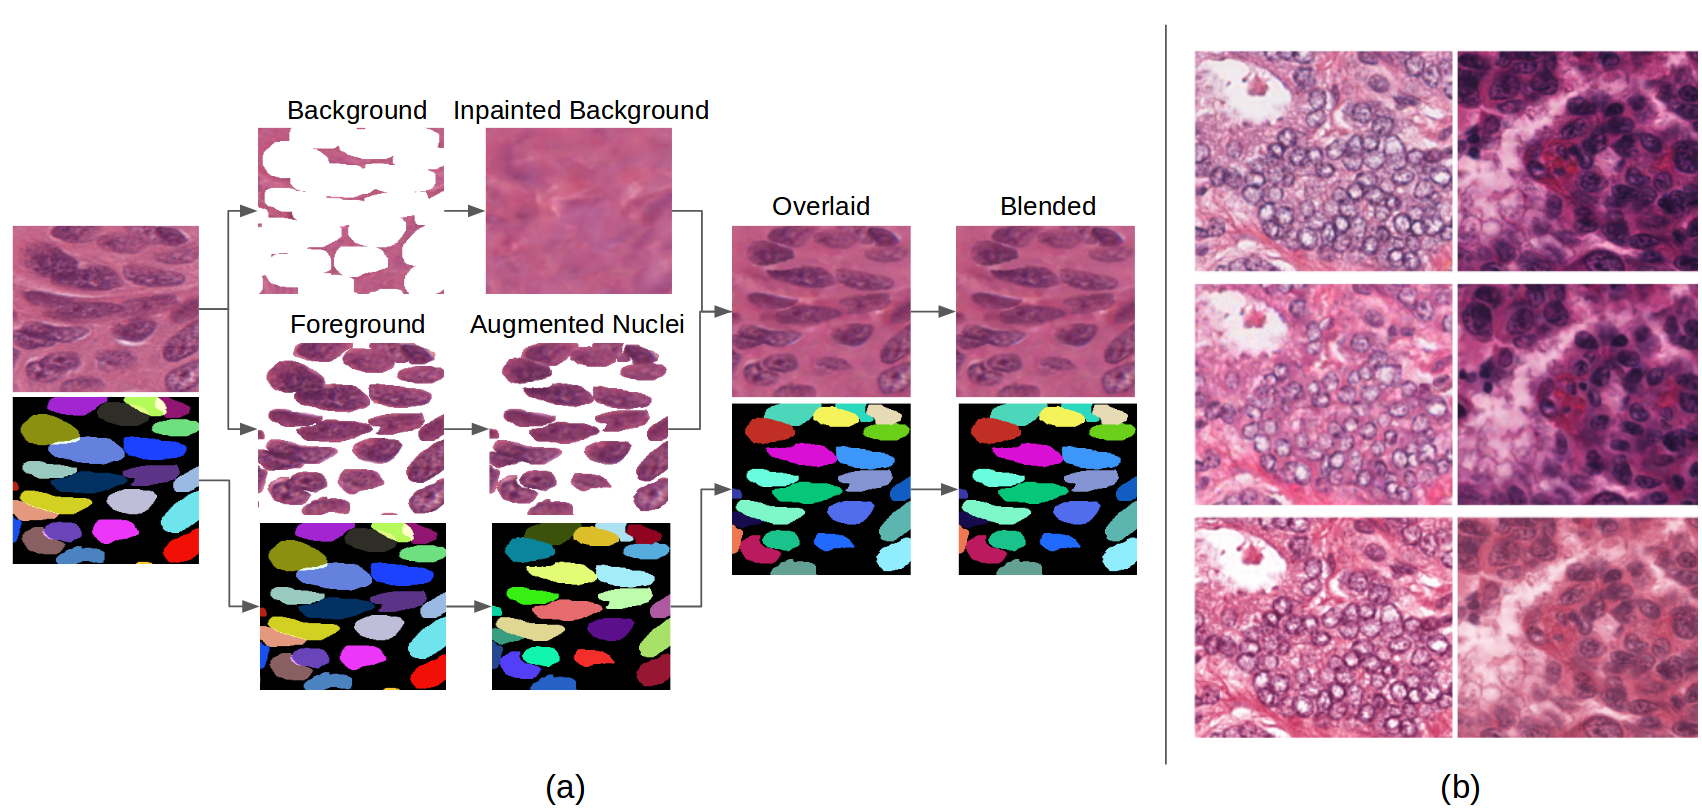
\includegraphics[width=\textwidth]{resources/4_data_augmentation.png}
    \caption{(a) Our proposed process generating new synthetic images with their corresponding annotations. 
    (b) Data augmentation and color normalization examples.
    The first row shows example training images from~\cite{he_dataset_kumar}.
    The second row shows synthetic images generated by our proposed data-augmentation method.
    %New shape and orientation of nuclei eyes generated along with translation, which increases the overlapping rate, make the training set more diverse. These new synthetic images have a significant contribution to the performance. 
    The last row shows the original training images normalized by the method proposed in~\cite{7164042}.
    %By converting all images to one color space, we can reduce the color variance problem, which alleviates the challenge when the model is trained.}
    }
    \label{fig:generate_new_data}
\end{figure}

\subsection{Data augmentation by nuclear deformation}

To aid in training a robust network that minimizes overfitting, we implemented a novel approach designed specific for histology image analysis to generate augmented training images.
Given the ground-truth annotations, each nucleus in an image is extracted and then deformed slightly by affine, spline, and elastic transformations as well as small random translation, yielding a new orientation, position, and shape.
Extracting the nucleus from the image produces empty holes in the background, which are filled by the image inpainting method proposed in~\cite{DBLP:journals/corr/abs-1801-07892}.
Some elastic transformations and slight Gaussian blurring are applied at this point, along with some added speckle noise.
The transformed nuclei are then overlaid back onto the reconstructed background image.
%We found that the signals of these cells are already smooth, so we do not need any blending method when placing these cells back to new background.
Finally Gaussian blurring is applied to help smooth any harsh or unnatural edges between the augmented nuclei and the background.
Figure~\ref{fig:generate_new_data} diagrams this process and shows examples of resulting augmented training images. 

\subsection{Stain normalization}
To reduce the uninformative and possibly confusing color variation inherent to H\&E stained images, we use the structure-preserving color normalization method proposed in~\cite{7164042}.
One image from the training data set is used as the target and all other images, including the new augmented data, are converted to its color space.
We use $\lambda = 0.1$ as recommended in~\cite{7164042}.
The last row in Figure~\ref{fig:generate_new_data}b shows example normalized images.


\begin{ChapAbstract}
In this chapter, we discuss the main challenges not only in nuclear segmentation but also other related domains such as astronomy analysis, video object segmentation. Moreover, we also describe the merit of our enhancements to overcome mentioned challenges, which can be extend to solve these problems in other fields.
\end{ChapAbstract}
